\documentclass{article}
\usepackage[utf8]{inputenc}
\usepackage[a4paper, total={6.5in, 9.5in}]{geometry}
\usepackage{graphicx} % Required for inserting images
\usepackage{enumitem}
\usepackage{booktabs,adjustbox}
\usepackage{multirow,multicol}
\usepackage{xcolor}
\usepackage{array,caption}
\usepackage{amssymb,amsmath}
\usepackage{ragged2e}
\usepackage{tikz,circuitikz}
\usepackage{titling}
\usepackage{hyperref}
\usepackage{tkz-euclide,subfigure}
\usepackage{subcaption}
\usepackage{nameref}
\captionsetup{font=Large}
	
\usetikzlibrary{shapes.geometric}
\usetikzlibrary{shapes,arrows,positioning,patterns,matrix,circuits.logic.IEC, calc}
\usepackage{pgfplots}
\pgfplotsset{compat=newest}
\usepgfplotslibrary{fillbetween,statistics}

\graphicspath{ {./Util/} }

\definecolor{blizzardblue}{rgb}{0.67, 0.9, 0.93}
\definecolor{bittersweet}{rgb}{1.0, 0.44, 0.37}
\definecolor{caribbeangreen}{rgb}{0.0, 0.8, 0.6}
\definecolor{carnationpink}{rgb}{1.0, 0.65, 0.79}
\definecolor{capri}{rgb}{0.0, 0.75, 1.0}
\definecolor{green(pigment)}{rgb}{0.0, 0.65, 0.31}
\definecolor{grannysmithapple}{rgb}{0.66, 0.89, 0.63}

% set spacing in tables
\setlength{\tabcolsep}{12pt}
\renewcommand{\arraystretch}{1.5}

\pretitle{\linespread{1.5}\huge}
\posttitle{\par\vspace{0.5cm}}

\title{
\begin{center}
CSE 300\\
Technical Writing and Presentation Sessional\\
Report: Maximum Bipartite Matching\\
Lab Section - A1\\
Group - 09\\
9th March, 2024
\end{center}
}
\author{}
\date{}

\begin{document}
\maketitle
\raggedright
\Large{Members of the Group:\par}
\Large{
\begin{enumerate}[label = \roman*.]
    \item 2005012 - Abrar Jahin Sarker
    \item 2005017 - Abdullah  Muhammed  Amimul Ehsan
    \item 2005020 - Mostafa Rifat Tazwar
\end{enumerate}
}
\newpage
\tableofcontents
\newpage
\section{Introduction}
\Large
The concept of maximum bipartite matching, a fundamental problem in graph theory, holds significant relevance across diverse fields due to its ability to model various real-world scenarios. Bipartite graphs serve as the foundational structure for this problem. In essence, a maximum bipartite matching seeks to pair elements from one subset with elements from the other subset in such a way that maximizes the number of paired elements. From applications in network flow optimization, job scheduling, and medical residency programs to its role in solving matching problems in societal contexts like marriage and kidney exchange programs, the utility of maximum bipartite matching extends across numerous domains, making it a subject of continued research and innovation.  
\subsection{Definitions}
\subsubsection{\large Bipartite Graph}
\Large
A bipartite graph is one whose vertices can be split into two independent groups U,V such that \textbf{every edge connects vertices of different groups.} \\
\vspace{10mm}
\begin{figure}[!h]
    \centering
    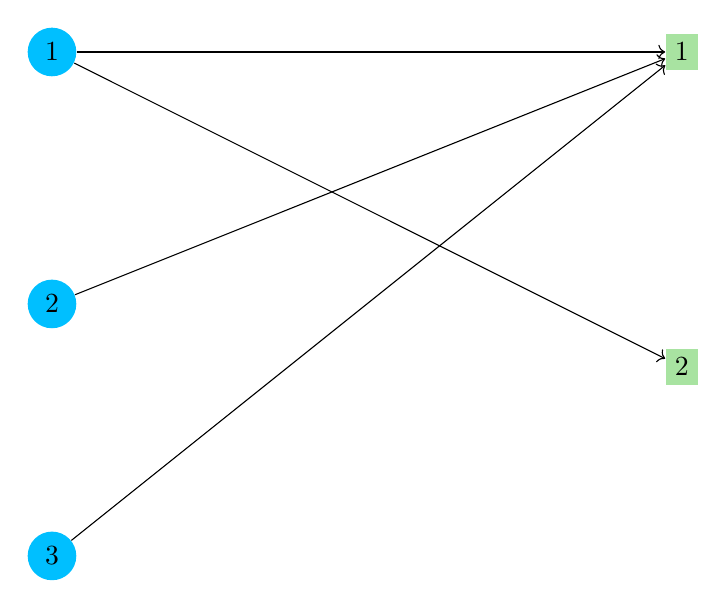
\begin{tikzpicture}[scale=4] 
        % 
        \node[fill=capri, circle] (b1) at (0,0) {1};
        \node[fill=capri, circle] (b2) at (0,-0.8) {2};
        \node[fill=capri, circle] (b3) at (0,-1.6) {3};
        
        % Girl
        \node[fill=grannysmithapple, rectangle] (g1) at (2,0) {1};
        \node[fill=grannysmithapple, rectangle] (g2) at (2,-1) {2};
        
        % Potential Pairs
        \draw[->] (b1) -- (g1);
        \draw[->] (b1) -- (g2);
        \draw[->] (b2) -- (g1);
        \draw[->] (b3) -- (g1);
        

    \end{tikzpicture}
    \caption{Visualization of bipartite graph}
\end{figure}
\newpage
\large \textbf{Properties of a Bipartite graph}\\
\Large
\begin{itemize}
    \item[-] There can \underline{not} be any edge between any two vertices of U or any two vertices of V .\\
    \item[-] The graph is \textcolor{blue}{two colourable} and doesn't have \textcolor{red}{cycles of odd length}.
\end{itemize}


\begin{figure}[!h]
    \centering
    \begin{tabular}{c c}
        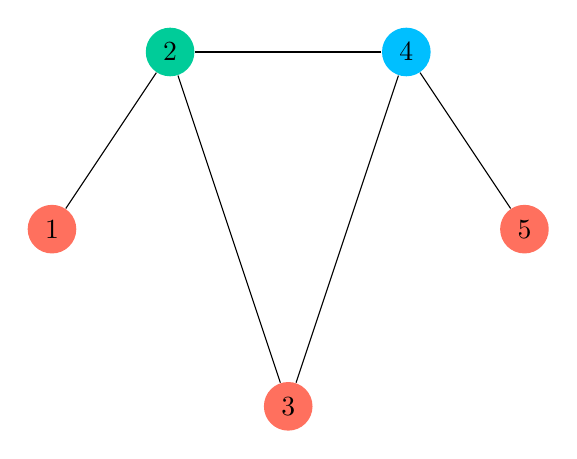
\begin{tikzpicture}[scale=1.5]
        
        
            \node[fill=bittersweet, circle] (r1) at (-0.75,0) {1} ;
            \node[fill=bittersweet, circle] (r3) at (1.25,-1.5) {3} ;
            \node[fill=bittersweet, circle] (r5) at (3.25,0) {5} ;
            \node[fill=caribbeangreen, circle] (g2) at (0.25,1.5) {2} ;
            \node[fill=capri, circle] (g4) at (2.25,1.5) {4} ;    
            
            \draw[-] (r1) -- (g2) ;
            \draw[-] (g2) -- (r3);
            \draw[-] (r3) -- (g4);
            \draw[-] (g4) -- (g2);
            \draw[-] (g4) -- (r5);
        
        
        
        \end{tikzpicture} & 
    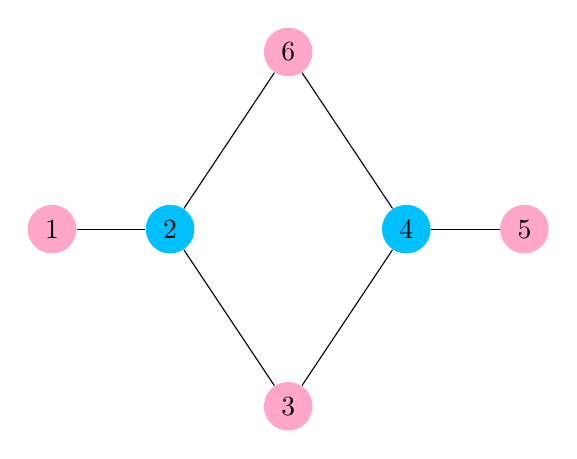
\begin{tikzpicture}[scale = 1.5]
        \node[fill=carnationpink, circle] (p1) at (-0.75,0) {1} ;
        \node[fill=carnationpink, circle] (p3) at (1.25,-1.5) {3} ;
        \node[fill=carnationpink, circle] (p6) at (1.25,1.5) {6} ;
        \node[fill=carnationpink, circle] (p5) at (3.25,0) {5} ;
        \node[fill=capri, circle] (b2) at (0.25,0) {2} ;
        \node[fill=capri, circle] (b4) at (2.25,0) {4} ;    
        
        \draw[-] (p1) -- (b2) ;
        \draw[-] (b2) -- (p3);
        \draw[-] (b2) -- (p6);
        \draw[-] (b4) -- (p3);
        \draw[-] (b4) -- (p6);
        \draw[-] (b4) -- (p5);
    \end{tikzpicture} \\
    Odd length cycle & Even length cycle \\
    Not 2 colorable & 2 colorable \\ 
    \textcolor{red}{Not a bipartite graph} &  \textcolor{caribbeangreen}{Bipartite graph}
    \end{tabular}
    \caption{Comparison between Bipartite and Non-bipartite graph}
\end{figure}

\subsubsection{\large Maximum Matching}
Given a bipartite graph, a matching is a subset of the edges for which \textbf{every vertex belongs to exactly one of the edges}. \par

And, a maximum matching is a matching of \textbf{maximum number of edges}. In a maximum matching, if any edge is added to it, it is no longer a matching.

\section{The Problem}
\textit{
Given a bipartite graph $G = (A \cup B, E)$, find an \{ $S \subseteq A \times B$ : $S$ is a matching and is as large as possible.} \} \cite{kleinberg2006algorithm}

\newpage

\section{Scenario}
In a picnic,there are 5 people and 5 food items.Some people express interest in some of the items.How can we satisfy \textbf{maximum number of people} while wasting \textbf{minimum number of items}?

\section{Greedy Approach}
Greedy approach seeks to find the \textbf{first available item} among the items in which the person is interested in and assigns that item to the person. Here's a simulation for the above scenario :- 

\begin{table}[!h]
    \centering
    \begin{tabular}{ccc}
      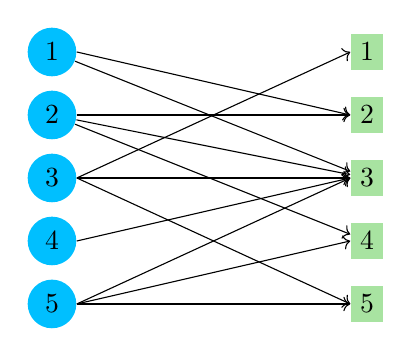
\begin{tikzpicture} 
            % 
            \node[fill=capri, circle] (p1) at (0,0) {1};
            \node[fill=capri, circle] (p2) at (0,-0.8) {2};
            \node[fill=capri, circle] (p3) at (0,-1.6) {3};
             \node[fill=capri, circle] (p4) at (0,-2.4) {4};
            \node[fill=capri, circle] (p5) at (0,-3.2) {5};
             
            
            
            % 
            \node[fill=grannysmithapple, rectangle] (f1) at (4,0) {1};
            \node[fill=grannysmithapple, rectangle] (f2) at (4,-0.8) {2};
            \node[fill=grannysmithapple, rectangle] (f3) at (4,-1.6) {3};
            \node[fill=grannysmithapple, rectangle] (f4) at (4,-2.4) {4};
            \node[fill=grannysmithapple, rectangle] (f5) at (4,-3.2) {5};
            
            % Potential Pairs
            \draw[->] (p1.east) -- (f2.west);
            \draw[->] (p1) -- (f3);
            \draw[->] (p2) -- (f2);
            \draw[->] (p2) -- (f3);
            \draw[->] (p2) -- (f4);
             \draw[->] (p3.east) -- (f1.west);
              \draw[->] (p3.east) -- (f3.west);
               \draw[->] (p3.east) -- (f5.west);
                \draw[->] (p4.east) -- (f3.west);
                  \draw[->] (p5.east) -- (f3.west);
               \draw[->] (p5.east) -- (f5.west);
                \draw[->] (p5.east) -- (f4.west);
            
            
            

        \end{tikzpicture} & 
        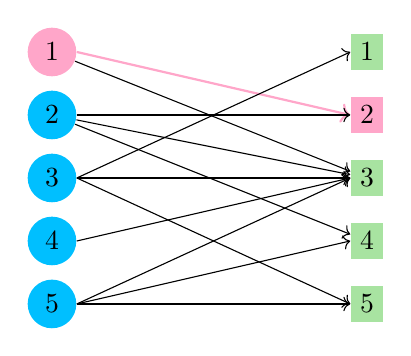
\begin{tikzpicture} 
            % 
            \node[fill=carnationpink, circle] (p1) at (0,0) {1};
            \node[fill=capri, circle] (p2) at (0,-0.8) {2};
            \node[fill=capri, circle] (p3) at (0,-1.6) {3};
             \node[fill=capri, circle] (p4) at (0,-2.4) {4};
            \node[fill=capri, circle] (p5) at (0,-3.2) {5}; 
            
            
            % 
            \node[fill=grannysmithapple, rectangle] (f1) at (4,0) {1};
            \node[fill=carnationpink, rectangle] (f2) at (4,-0.8) {2};
            \node[fill=grannysmithapple, rectangle] (f3) at (4,-1.6) {3};
            \node[fill=grannysmithapple, rectangle] (f4) at (4,-2.4) {4};
            \node[fill=grannysmithapple, rectangle] (f5) at (4,-3.2) {5};
        
            
            % Potential Pairs
           \draw[carnationpink,thick,->] (p1.east) --  (f2.west);
            \draw[->] (p1) -- (f3);
            \draw[->] (p2) -- (f2);
            \draw[->] (p2) -- (f3);
            \draw[->] (p2) -- (f4);
             \draw[->] (p3.east) -- (f1.west);
              \draw[->] (p3.east) -- (f3.west);
               \draw[->] (p3.east) -- (f5.west);
                \draw[->] (p4.east) -- (f3.west);
                  \draw[->] (p5.east) -- (f3.west);
               \draw[->] (p5.east) -- (f5.west);
                \draw[->] (p5.east) -- (f4.west);
            
            
            

        \end{tikzpicture} & 
        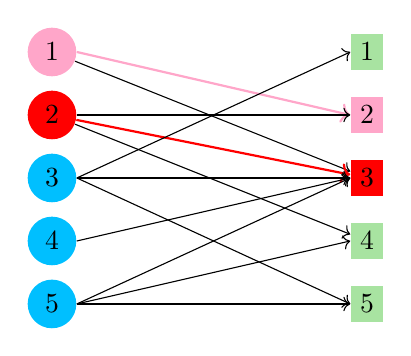
\begin{tikzpicture} 
            % 
            \node[fill=carnationpink, circle] (p1) at (0,0) {1};
            \node[fill=red, circle] (p2) at (0,-0.8) {2};
            \node[fill=capri, circle] (p3) at (0,-1.6) {3};
             \node[fill=capri, circle] (p4) at (0,-2.4) {4};
            \node[fill=capri, circle] (p5) at (0,-3.2) {5};
             
            
            
            % 
            \node[fill=grannysmithapple, rectangle] (f1) at (4,0) {1};
            \node[fill=carnationpink, rectangle] (f2) at (4,-0.8) {2};
            \node[fill=red, rectangle] (f3) at (4,-1.6) {3};
            \node[fill=grannysmithapple, rectangle] (f4) at (4,-2.4) {4};
            \node[fill=grannysmithapple, rectangle] (f5) at (4,-3.2) {5};
            
            % Potential Pairs
           \draw[carnationpink,thick,->] (p1.east) --  (f2.west);
            \draw[->] (p1) -- (f3);
            \draw[->] (p2) -- (f2);
            \draw[red,thick,->] (p2) -- (f3);
            \draw[->] (p2) -- (f4);
             \draw[->] (p3.east) -- (f1.west);
              \draw[->] (p3.east) -- (f3.west);
               \draw[->] (p3.east) -- (f5.west);
                \draw[->] (p4.east) -- (f3.west);
                  \draw[->] (p5.east) -- (f3.west);
               \draw[->] (p5.east) -- (f5.west);
                \draw[->] (p5.east) -- (f4.west);
            
            
            

        \end{tikzpicture} \\
        (a) & (b) & (c) \\ \hline
        & & \\
        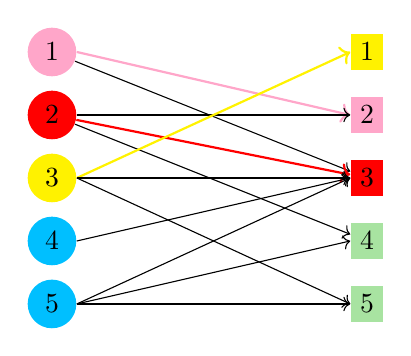
\begin{tikzpicture} 
            % 
            \node[fill=carnationpink, circle] (p1) at (0,0) {1};
            \node[fill=red, circle] (p2) at (0,-0.8) {2};
            \node[fill=yellow, circle] (p3) at (0,-1.6) {3};
             \node[fill=capri, circle] (p4) at (0,-2.4) {4};
            \node[fill=capri, circle] (p5) at (0,-3.2) {5};
             
            
            
            % 
            \node[fill=yellow, rectangle] (f1) at (4,0) {1};
            \node[fill=carnationpink, rectangle] (f2) at (4,-0.8) {2};
            \node[fill=red, rectangle] (f3) at (4,-1.6) {3};
            \node[fill=grannysmithapple, rectangle] (f4) at (4,-2.4) {4};
            \node[fill=grannysmithapple, rectangle] (f5) at (4,-3.2) {5};
            
            % Potential Pairs
           \draw[carnationpink,thick,->] (p1.east) --  (f2.west);
            \draw[->] (p1) -- (f3);
            \draw[->] (p2) -- (f2);
            \draw[red,thick,->] (p2) -- (f3);
            \draw[->] (p2) -- (f4);
             \draw[yellow,thick,->] (p3.east) -- (f1.west);
              \draw[->] (p3.east) -- (f3.west);
               \draw[->] (p3.east) -- (f5.west);
                \draw[->] (p4.east) -- (f3.west);
                  \draw[->] (p5.east) -- (f3.west);
               \draw[->] (p5.east) -- (f5.west);
                \draw[->] (p5.east) -- (f4.west);
            
            
            

        \end{tikzpicture} &
        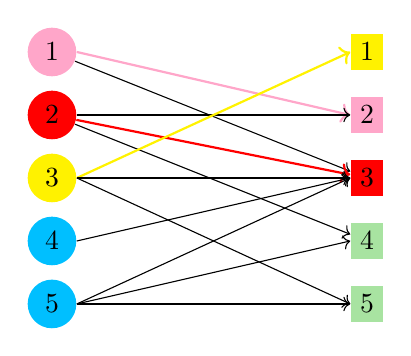
\begin{tikzpicture} 
            % 
            \node[fill=carnationpink, circle] (p1) at (0,0) {1};
            \node[fill=red, circle] (p2) at (0,-0.8) {2};
            \node[fill=yellow, circle] (p3) at (0,-1.6) {3};
             \node[fill=capri, circle] (p4) at (0,-2.4) {4};
            \node[fill=capri, circle] (p5) at (0,-3.2) {5};
             
            
            
            % 
            \node[fill=yellow, rectangle] (f1) at (4,0) {1};
            \node[fill=carnationpink, rectangle] (f2) at (4,-0.8) {2};
            \node[fill=red, rectangle] (f3) at (4,-1.6) {3};
            \node[fill=grannysmithapple, rectangle] (f4) at (4,-2.4) {4};
            \node[fill=grannysmithapple, rectangle] (f5) at (4,-3.2) {5};
            
            % Potential Pairs
           \draw[carnationpink,thick,->] (p1.east) --  (f2.west);
            \draw[->] (p1) -- (f3);
            \draw[->] (p2) -- (f2);
            \draw[red,thick,->] (p2) -- (f3);
            \draw[->] (p2) -- (f4);
             \draw[yellow,thick,->] (p3.east) -- (f1.west);
              \draw[->] (p3.east) -- (f3.west);
               \draw[->] (p3.east) -- (f5.west);
                \draw[->] (p4.east) -- (f3.west);
                  \draw[->] (p5.east) -- (f3.west);
               \draw[->] (p5.east) -- (f5.west);
                \draw[->] (p5.east) -- (f4.west);
            
            
            

        \end{tikzpicture} &
        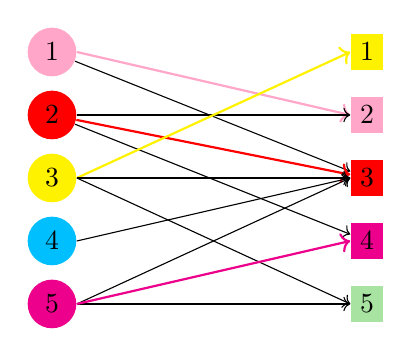
\begin{tikzpicture} 
            % 
            \node[fill=carnationpink, circle] (p1) at (0,0) {1};
            \node[fill=red, circle] (p2) at (0,-0.8) {2};
            \node[fill=yellow, circle] (p3) at (0,-1.6) {3};
             \node[fill=capri, circle] (p4) at (0,-2.4) {4};
            \node[fill=magenta, circle] (p5) at (0,-3.2) {5};
             
            
            
            % 
            \node[fill=yellow, rectangle] (f1) at (4,0) {1};
            \node[fill=carnationpink, rectangle] (f2) at (4,-0.8) {2};
            \node[fill=red, rectangle] (f3) at (4,-1.6) {3};
            \node[fill=magenta, rectangle] (f4) at (4,-2.4) {4};
            \node[fill=grannysmithapple, rectangle] (f5) at (4,-3.2) {5};
            
            % Potential Pairs
           \draw[carnationpink,thick,->] (p1.east) --  (f2.west);
            \draw[->] (p1) -- (f3);
            \draw[->] (p2) -- (f2);
            \draw[red,thick,->] (p2) -- (f3);
            \draw[->] (p2) -- (f4);
             \draw[yellow,thick,->] (p3.east) -- (f1.west);
              \draw[->] (p3.east) -- (f3.west);
               \draw[->] (p3.east) -- (f5.west);
                \draw[->] (p4.east) -- (f3.west);
                  \draw[->] (p5.east) -- (f3.west);
               \draw[->] (p5.east) -- (f5.west);
                \draw[magenta,thick,->] (p5.east) -- (f4.west);
            
            
            

        \end{tikzpicture} 
        \\
        (d) & (e) & (f) \\ \hline
    \end{tabular}
    \caption*{
    a) We define the problem using a graph, where any \textcolor{blue}{blue} vertex represents a person to whom no item has been assigned and any \textcolor{caribbeangreen}{green} vertex represents the items available. Edges from a person to an item depicts their interest in that item.
    \\ b) Person 1 initiates the process by selecting the first available item (item 2).
	\\ c) Person 2's only viable option is item 3, as item 2 has already been chosen.
	\\ d) Person 3 selects item 3.
	\\ e) Person 4 cannot be assigned an item, as all options previously chosen by them have been allocated.
	\\ f) Person 5 discovers that item 4 is available for selection.
	}
    \label{tab:greedy_approch}
\end{table}
\textit{Bipartite matching : }  \{(1, 2), (2, 3), (3, 1), (5, 4)\}\\

Although greedy provides us with a valid matching , it is not maximal.

\section{References}
\bibliographystyle{plain}
\bibliography{ref}

\end{document}